% !TEX encoding = UTF-8
\documentclass[xcolor=dvipsnames]{beamer}

\usepackage{lmodern}
\usepackage[ngerman]{babel}
\usepackage[utf8]{inputenc}
\usepackage{color}
\usepackage{graphicx}

\usetheme{CambridgeUS}
\usecolortheme{seahorse}
\useinnertheme{rectangles}
\setbeamertemplate{blocks}[rounded][shadow=false]



\beamertemplatenavigationsymbolsempty



\title{{\scriptsize{MA2STT2004 - Projektmodul\newline
\\\emph{Praxis der Digital Humanities}
\\Prof. Dr. Caroline Sporleder}}
\newline\\\textcolor{black}{\huge{Projektgruppe 2\newline
}}}
\author{C. Ahrens, A. Beyer, C. Michels}
\institute{Fachbereich II --  Computerlinguistik und Digital Humanities
\newline\\Universität Trier}
\date{\today}
%\logo{\includegraphics[scale=0.14]{logo-SF}}



\begin{document}

\begin{frame}[plain]
\titlepage
\end{frame}

\title{Projektgruppe 2}
\institute{}

\begin{frame}[plain]\frametitle{\textcolor{black}{Übersicht}}
\tableofcontents[hideallsubsections]
\end{frame}

%###########################################################################
%%%%%%%%%%%%%%%%%%%%%%%%%%%%%%%%%%%%%%%%%%%%%%%%%%%%%%%%
%###########################################################################

\section{Ansätze zur Koreferenzresolution}

%###########################################################################

\subsection{Barth}

%---

\begin{frame}[plain]\frametitle{\textcolor{black}{Übersicht}}

\tableofcontents[currentsection, hideothersubsections]

\end{frame}

\addtocounter{framenumber}{-3}

%---

\begin{frame}\frametitle{\textcolor{black}{Was ist Barth 2.0?}}

\begin{block}{Barth}
\begin{itemize}
\item Barth
\begin{itemize}
\item Barth
\end{itemize}
\item Barth
\item Barth
\end{itemize}
\end{block}

\end{frame}

%###########################################################################

\subsection{Reconcile}
%--- 

\begin{frame}\frametitle{\textcolor{black}{Was ist Reconcile?}}

\begin{block}{Reconcile}
\begin{itemize}
  \item Framework für Koreferenzen
  \item Baukasten aus diversen Systemen
  \item eigene Erweiterungen
\end{itemize}
\end{block}

\end{frame}

\begin{frame}\frametitle{\textcolor{black}{Was ist das Problem mit Reconcile?}}

\begin{block}{Probleme}
\begin{itemize}
  \item Keine Dokumentation
  \item Ich wurde auf der Mailingliste abgelehnt
  \item Die einzige Beispielanwendung war aus der CONLL Aufgabe
\end{itemize}
\end{block}

\end{frame}


%###########################################################################

\subsection{DCoref}
%--- 

\begin{frame}\frametitle{\textcolor{black}{Was ist DCoref?}}

\begin{block}{DCoref}
\begin{itemize}
\item deterministisches Modul der Stanford CoreNLP
\begin{itemize}
\item hängt von anderen Modulen ab (pos, lemma, ner, parse)
\item diese Module müssen in der Pipeline vorher angewendet werden
\end{itemize}
\item arbeitet mit Sieben
\begin{itemize}
\item erste Stufe: bevorzugt Recall (detection)
\item zweite Stufe: Siebe bevorzugen Precision
\end{itemize} 
\item Post-Processing: mehr Precision (?)
\end{itemize}
\end{block}

\end{frame}

%###########################################################################
%%%%%%%%%%%%%%%%%%%%%%%%%%%%%%%%%%%%%%%%%%%%%%%%%%%%%%%%
%###########################################################################

\section{Verlauf}

%###########################################################################

\subsection{Vergleichen}

%---

\begin{frame}[plain]\frametitle{\textcolor{black}{Übersicht}}

\tableofcontents[currentsection, hideothersubsections]

\end{frame}

\addtocounter{framenumber}{-1}

%--- 

\begin{frame}\frametitle{\textcolor{black}{Suche nach dem besten Ansatz}}

\begin{block}{Vergleichsgegenstände}
\begin{itemize}
\item Reconcile
\item DCoref
\end{itemize}
\end{block}

\begin{block}{Ohne Barth}
\begin{itemize}
\item nur Reintext als Eingabe
\item Zeitgründe
\end{itemize}
\end{block}

\begin{block}{Vergleichspunkte}
\begin{itemize}
\item Precision
\item Recall
\item FScore
\end{itemize}
\end{block}

\end{frame}

%--- 

\begin{frame}\frametitle{\textcolor{black}{Suche nach dem besten Ansatz}}

\begin{block}{Werkzeug: MMAX}
\begin{itemize}
\item Schwierigkeiten bei der Verwendung
\begin{itemize}
\item Vergleich war entsprechend auch schwierig/unmöglich
\end{itemize}
\end{itemize}
\end{block}

\begin{block}{Testdaten: Uncle Tom's Cabin}
\begin{itemize}
\item erste Hälfte des ersten Kapitels, Reintext
\begin{itemize}
\item bis zu dem Wort \emph{Wilberforce}
\item eindeutige Grenze
\end{itemize}
\end{itemize}
\end{block}

\end{frame}

%--- 

\begin{frame}\frametitle{\textcolor{black}{{MMAX - Beispiel der Anzeige}}}
\begin{figure}
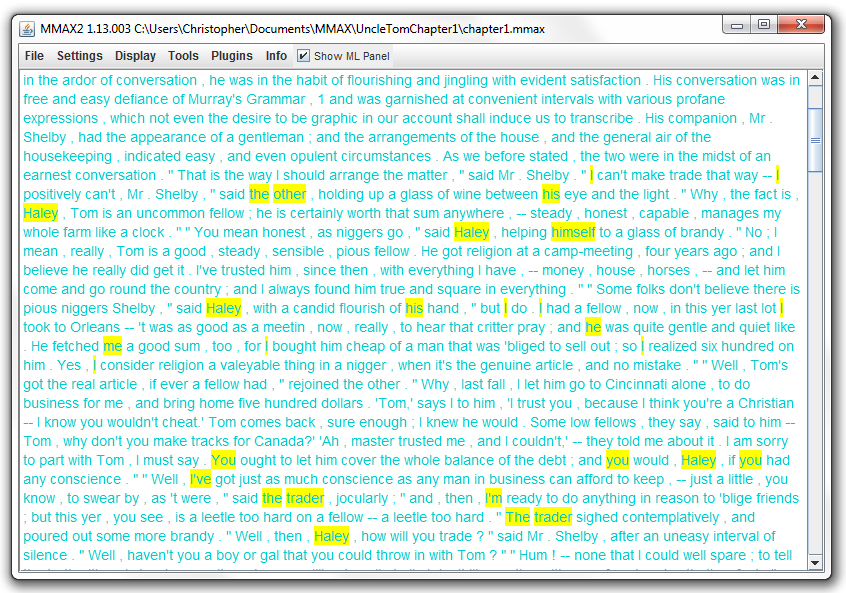
\includegraphics[height=7.25cm]{cm_mmax.jpg}
\end{figure}

\end{frame}

\begin{frame}\frametitle{\textcolor{black}{{Standartweg: ConLL}}}
\begin{figure}
  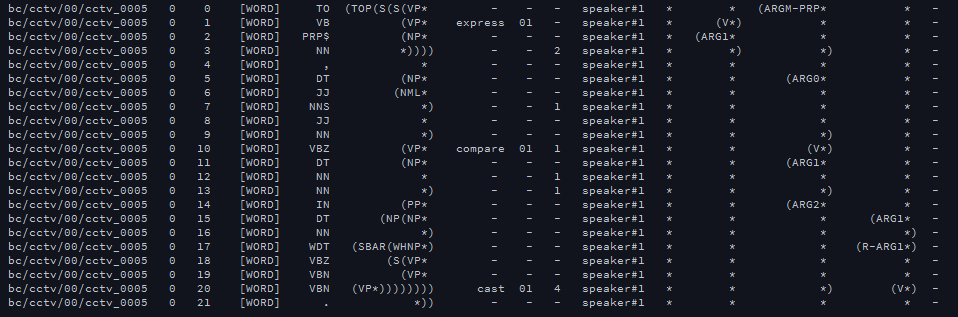
\includegraphics[width=11cm]{img/conll.png}
\end{figure}

\end{frame}

%--- 

\begin{frame}\frametitle{\textcolor{black}{Fortsetzung der Suche ohne MMAX}}

\begin{block}{Standard finden ohne Werkzeug}
\begin{itemize}
\item Reconcile-Ausgabe für Testdaten als Ausgangspunkt
\item korrigierte Version von zwei Annotatoren im gleichen Format erstellt
\begin{itemize}
\item DCoref-Ausgabeformat umgewandelt in Reconcile-Ausgabeformat
\end{itemize}
\end{itemize}
\end{block}

\begin{block}{Scorer für Reconcile-Ausgabe}
\begin{itemize}
\item wird für beide korrigierten Versionen verwendet
\item Ergebnisse:
\end{itemize}
\begin{center}
  \begin{tabular}{ l || c | c | c ||  r }
				& Reconcile 	& DCoref 	& DCoref (PP) 	& \\ \hline \hline
    	Precision 	& 0.99673 	& 0.74510	& 0.74837		& \\ \hline
    	Recall     	& 0.97917 	& 0.35775 	& 0.33861 		& \\ \hline
    	FScore    	& 0.98787  	& 0.48340 	& 0.46625 		& \\ \hline
  \end{tabular}
\end{center}
\end{block}

\end{frame}

%###########################################################################


\subsection{Formatieren}

%---

\begin{frame}\frametitle{\textcolor{black}{Formatieren: Reconcile}}

  \begin{center}
    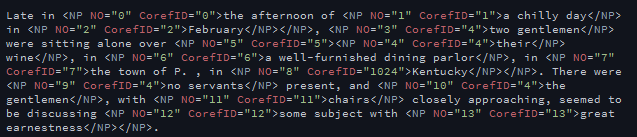
\includegraphics[width=11cm]{img/reconcile-output.png}
  \end{center}
  
\end{frame}

\begin{frame}\frametitle{\textcolor{black}{Formatieren: Reconcile}}

  \begin{center}
    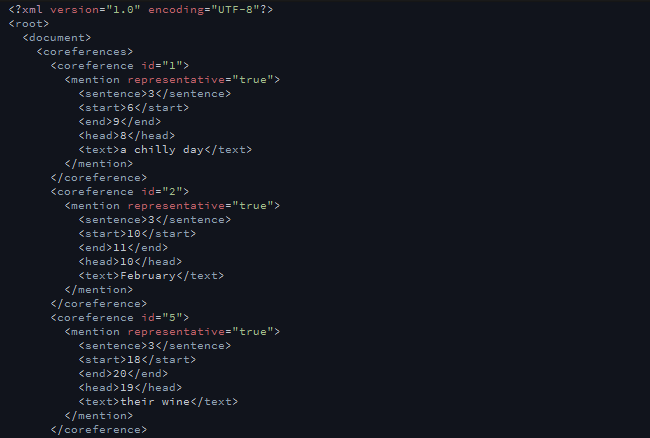
\includegraphics[width=11cm]{img/xml-format-1.png}
  \end{center}
  
\end{frame}

\begin{frame}\frametitle{\textcolor{black}{Formatieren: Reconcile}}

  \begin{center}
    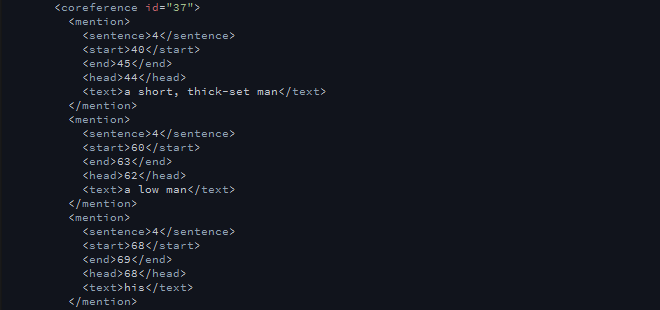
\includegraphics[width=11cm]{img/xml-format-2.png}
  \end{center}

\end{frame}

%---

\begin{frame}[fragile]\frametitle{\textcolor{black}{Formatieren: DCoref}}

\begin{block}{DCoref - Input}
\begin{itemize}
\item Reintext
\begin{verbatim}
And the trader leaned back in his chair, and folded  
his arm, with an air of virtuous decision, apparently
considering himself a second Wilberforce. 
\end{verbatim}
\end{itemize}
\end{block}



\end{frame}

%---

\begin{frame}[fragile]\frametitle{\textcolor{black}{Formatieren: DCoref}}

\begin{block}{DCoref - Output}
\begin{itemize}
\item unformatiert: XML
\begin{small}\begin{verbatim}
<?xml version="1.0" encoding="UTF-8"?>
<?xml-stylesheet href="CoreNLP-to-HTML.xsl" type="text/xsl"?>
<root>
  <document>
    <sentences/>
    <coreference>
      <coreference>
        <mention representative="true"/>
        <mention/>
      </coreference>
      <coreference/>
    </coreference>
  </document>
</root>
\end{verbatim}
\end{small}
\end{itemize}
\end{block}

\end{frame}

%---

\begin{frame}[fragile]\frametitle{\textcolor{black}{Formatieren: DCoref}}

\begin{block}{DCoref - Output}
\begin{itemize}
\item formatiert für Gruppe 3: XML
\begin{small}\begin{verbatim}
<?xml version="1.0" encoding="UTF-8" standalone="no"?>
<chapter id="1" title="In Which [...] Humanity">
  <sentences/>
  <coreferences>
    <coreference id="1">
      <mention representative="true">
      <mention/>
    </coreference>
    <coreference/>
  </coreferences>
</chapter>
\end{verbatim}
\end{small}
\end{itemize}
\end{block}

\end{frame}

%###########################################################################


\subsection{Indizieren}

%---

\begin{frame}[fragile]\frametitle{\textcolor{black}{Indizieren: Letzter Schritt zur endgültigen Ausgabe}}

\begin{block}{Index - Input}
\begin{itemize}
\item für Gruppe 3 formatierte XML-Dateien für alle Kapitel: 
\begin{small}\begin{verbatim}
<?xml version="1.0" encoding="UTF-8" standalone="no"?>
<chapter id="1" title="In Which [...] Humanity">
  <sentences/>
  <coreferences>
    <coreference id="1">
      <mention representative="true">
      <mention/>
    </coreference>
    <coreference/>
  </coreferences>
</chapter>
\end{verbatim}
\end{small}
\end{itemize}
\end{block}

\end{frame}

\begin{frame}[fragile]\frametitle{\textcolor{black}{Indizieren: Letzter Schritt zur endgültigen Ausgabe}}

\begin{block}{Index - Output}
\begin{itemize}
\item für Gruppe 3 formatierte XML-Datei als Nachschlagewerk
\begin{itemize}
\item Nachschlagewerk für kapitelübergreifende Ketten
\end{itemize}
\begin{small}\begin{verbatim}
<?xml version="1.0" encoding="UTF-8"?>
<root>
  <chains>
    <chain text="these two">
      <coreference>
        <id>38</id>
        <chapter>37</chapter>
      </coreference>
      <coreference>
        <id>86</id>
        <chapter>5</chapter>
      </coreference>
    </chain>
    <chain/>
  </chains>
</root>
\end{verbatim}
\end{small}
\end{itemize}
\end{block}

\end{frame}

%###########################################################################
%%%%%%%%%%%%%%%%%%%%%%%%%%%%%%%%%%%%%%%%%%%%%%%%%%%%%%%%
%###########################################################################

\section{Demonstration}

%###########################################################################

\subsection{Reconcile}

%---

\begin{frame}[plain]\frametitle{\textcolor{black}{Übersicht}}

\tableofcontents[currentsection, hideothersubsections]

\end{frame}

\addtocounter{framenumber}{-1}

%--- 

\begin{frame}\frametitle{\textcolor{black}{``{Version Space (Angepasst)}''. \emph{Wikimedia Commons}.}}
\begin{figure}
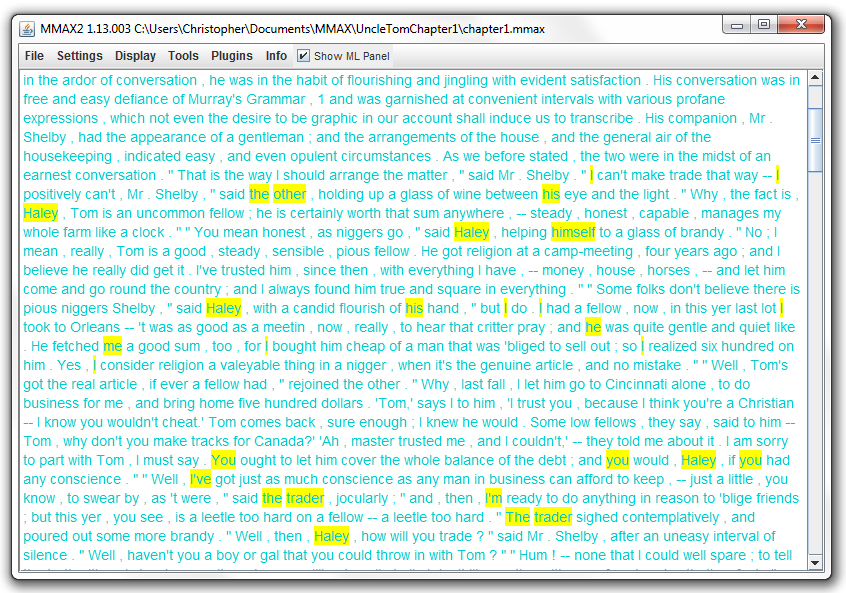
\includegraphics[height=7cm]{cm_mmax.jpg}
\end{figure}

\end{frame}

%###########################################################################

\subsection{DCoref}

%--- 

\begin{frame}[fragile]\frametitle{\textcolor{black}{Ausführoptionen von coref-adder.jar}}

\begin{block}{Hilfetext}
\begin{itemize}
\item Welche Optionen gibt es?
\begin{scriptsize}\begin{verbatim}
C:\project\folder>java -jar coref-adder.jar -help
usage: arguments for coref-adder.jar
 -corenlp               run Stanford CoreNLP first (optional)
 -folder <src-folder>   use given folder as source (required)
 -help                  print this message
 -pp                    include post-processing for DCoref in the CoreNLP
                        pipeline, ignored if -corenlp is not chosen
                        (optional)
C:\project\folder>
\end{verbatim}
\end{scriptsize}
\end{itemize}
\end{block}

\begin{block}{Wie führe ich ``coref-adder.jar'' aus?}
\end{block}

\end{frame}

%###########################################################################

\subsection{Indizierung}

%--- 

\begin{frame}\frametitle{\textcolor{black}{``{Version Space (Angepasst)}''. \emph{Wikimedia Commons}.}}
\begin{figure}
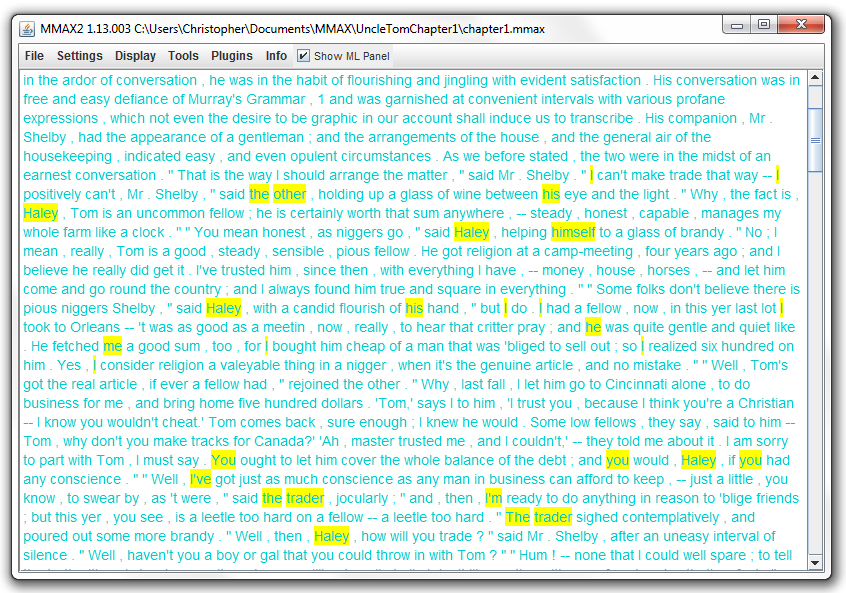
\includegraphics[height=7cm]{cm_mmax.jpg}
\end{figure}

\end{frame}

\addtocounter{framenumber}{-3}

%---

\begin{frame}[plain]
\frametitle{\textcolor{black}{Zeit für Fragen}}
Gibt es noch offene Fragen oder Dinge, die unklar geblieben sind?
\end{frame}

%% \begin{frame}[plain]
%% \frametitle{\textcolor{black}{Zum Schluss}}
%% Vielen Dank für eure Aufmerksamkeit!
%% \end{frame}

%\begin{frame}[plain]
%\frametitle{\textcolor{black}{Literatur}}
%\begin{thebibliography}{9}
%\bibitem[Mitchell]{buch} Mitchell, Tom M. (1982). ``Generalization as search". \emph{Artificial Intelligence} 18 (2): 203–226.
%\bibitem[Rendell]{buch} Rendell, Larry (1986). ``A general framework for induction and a study of selective induction". \emph{Machine Learning} 1 (2): 177–226.
%\bibitem[Sverdlik]{buch} Sverdlik, W.; Reynolds, R.G. (1992). ``Dynamic version spaces in machine learning". Proceedings, \emph{Fourth International Conference on Tools with Artificial Intelligence (TAI '92)}. Arlington, VA. pp. 308–315.
%\end{thebibliography}
%\end{frame}



\end{document}
